\documentclass[11pt]{article}

\usepackage[a4paper,margin=1in]{geometry}
\usepackage{amsmath,amssymb}
\usepackage{booktabs}
\usepackage{graphicx}
\usepackage[font=footnotesize,labelfont=footnotesize]{caption}
\usepackage[colorlinks=true,linkcolor=blue,citecolor=blue,urlcolor=blue]{hyperref}
\usepackage{parskip}
\newcommand{\SI}[2]{#1\,#2}
\newcommand{\vx}{\mathbf{x}}
\newcommand{\vW}{\mathbf{W}}

\title{Adaptive Vibration Cancellation in SPECULA:\\
implementation, simulation and analysis}
\author{Marco Falotico\\}
\date{\today}

\begin{document}
\maketitle

% \begin{abstract}
% This report documents the implementation of the Adaptive Vibration Cancellation (AVC) algorithm of Muradore, Pettazzi, Fedrigo \& Clare (SPIE 8447-38) as a SPECULA processing object, its behaviour in a full closed-loop adaptive-optics simulation, and an analysis of why parts of the algorithm work while others cannot.
%
% In its best configuration the module removes a \SI{47}{Hz} tip vibration almost completely: the mode-0 residual falls from \SI{630}{nm} to \SI{27}{nm} RMS ($-96\%$) and the vibration line is suppressed by \SI{63}{dB}.
%
% We then show that the plant-identification half of the algorithm is ill-posed --- a single tone cannot excite four parameters --- and that the cost function being minimized is an equation-error, not a control error, to the point of being independent of the parameters it is supposed to optimise.
%
% The practical conclusion is that the plant response should be calibrated and frozen, while the frequency and the disturbance quadratures are estimated online.
% \end{abstract}

\tableofcontents

\section{The algorithm}
\label{sec:alg}

The AVC module of Muradore et al.~\cite{muradore2012} is designed to sit \emph{in parallel} with an existing AO controller and remove one narrowband vibration, without requiring the main loop to be retuned.
%
It targets vibrations above the loop bandwidth, where the rejection transfer function of a classical integrator amplifies rather than attenuates.

\subsection{State and control law}

Each AVC instance tracks one tone and carries four adapted numbers,
%
\begin{equation}
  \vx=(x_1,x_2,x_3,x_4)^\top=(P_R,\;P_I,\;\lambda_c,\;\lambda_s)^\top,
\end{equation}
%
interpreted by the paper as the real and imaginary parts of the plant frequency response at the vibration frequency, and the cosine/sine quadratures of the disturbance.
%
It is convenient to group them into two complex numbers,
%
\begin{equation}
  P=x_1+ix_2 \quad(\text{plant}),
  \qquad
  \Lambda=x_3+ix_4 \quad(\text{disturbance}).
\end{equation}
%
Three conventions are used throughout. An overbar denotes complex
conjugation, $\overline{P}=x_1-ix_2$; a hat denotes a quantity held by the
algorithm as an estimate, $\hat P$ and $\hat\Lambda$; and a star denotes
the corresponding true value of the physical system, $P_\star$ and
$\Lambda_\star$. The distinction between $\hat P$ and $P_\star$ matters
from Sec.~\ref{sec:analysis} onwards, where the question is precisely
whether the former can be made to approach the latter.
%
From these the algorithm forms the control quadratures $\vartheta=\theta_c+i\theta_s$, with
%
\begin{equation}
  \theta_c=-\frac{x_1x_3-x_2x_4}{D},
  \qquad
  \theta_s=-\frac{x_1x_4+x_2x_3}{D},
  \qquad
  D \;=\; x_1^2+x_2^2+\epsilon \;=\; |P|^2+\epsilon ,
  \label{eq:theta}
\end{equation}
%
which in complex form is simply
\begin{equation}
  \vartheta=-\frac{P\,\Lambda}{D}
  \qquad\xrightarrow[\;\epsilon\to0\;]{}\qquad
  \vartheta=-\frac{\Lambda}{\overline{P}} ,
  \label{eq:thetacomplex}
\end{equation}
the first form following from $P\Lambda=(x_1x_3-x_2x_4)+i(x_1x_4+x_2x_3)$,
and the limit from $D\to|P|^2=P\overline{P}$ as $\epsilon\to0$.
%
The algorithm computes the correction $u(t)=\theta_c\cos\alpha+\theta_s\sin\alpha$, where $\alpha$ is the running phase estimate.
%
The idea is to cancel the disturbance $\Lambda$ by applying a command that is the estimate of the input vibration multiplied by the inverse of the plant response, so that the sum of the command and the disturbance is zero at the sensor.

\paragraph{The regularizer $\epsilon$.}
The quantity $\epsilon\ge0$ in \eqref{eq:theta} requires a note, because it is not part of the published algorithm.
%
The paper divides by $x_1^2+x_2^2$ exactly, i.e.\ $\epsilon=0$.
%
That denominator is the squared magnitude of the \emph{plant estimate}, so the commanded amplitude diverges whenever the estimate approaches the origin and, nothing in the update law prevents it from going to infinity.
%
Implementations therefore guard the division.
%
ESO's \textit{updateAVC.m} freezes $\vartheta$ to $(1,0)$ whenever $x_1^2+x_2^2<\theta_{\min}$ with $\theta_{\min}=10^{-2}$: this is a \emph{discontinuous} clamp, which in our simulations caused the states to jump between the boundary clip values.
%
A smooth equivalent is also implemented, $D=|P|^2+\epsilon$ with $\epsilon=\theta_{\min}$, which bounds the commanded amplitude by $\sim\!1/\epsilon$.
%
In the end, $\epsilon$ is a numerical safeguard with an arbitrary value.

\subsection{Adaptation}

With $c := \cos\alpha$, $s := \sin\alpha$ the algorithm defines the
regressor and the prediction error
\begin{equation}
  \vW=\big(\theta_cc+\theta_ss,\;\;\theta_sc-\theta_cs,\;\;c,\;\;s\big)^\top,
  \qquad
  e=\vW^\top\vx-y ,
  \label{eq:W}
\end{equation}
$y$ being the measured residual of the mode of interest, and updates the
state as:
\begin{equation}
  \vx \leftarrow \vx-\mu\,\vW\,e,
  \qquad \mu=g_xT_s .
  \label{eq:update}
\end{equation}
A separate phase-locked loop tracks the vibration
frequency~\cite{gardner2005,lindsey1981}, following the direct
(PLL-based) scheme of Bodson and Douglas~\cite{bodson1997}:
\begin{equation}
  \omega\leftarrow\omega+2g_\omega T_s\sin\alpha\;e,
  \qquad
  \alpha\leftarrow\alpha+T_s\omega+2kg_\omega T_s\sin\alpha\;e .
  \label{eq:pll}
\end{equation}
%
% Note the sign: the frequency loop is driven by $+e$ while the state update
% \eqref{eq:update} uses $-e$. This is explicit in \textit{updateAVC.m} and is
% reproduced by the SPECULA object; getting it wrong turns the phase detector
% into positive feedback and the loop never acquires.

The algorithm performs two online updates: an estimate of the plant response at the vibration frequency ($x_1,x_2$) and an estimate of the disturbance quadratures ($x_3,x_4$).
%
In parallel to these, the PLL tracks the vibration frequency and phase.
%
The gains $g_x$ and $g_\omega$ set the adaptation rates of the plant/disturbance and the PLL, respectively.

\subsection{Implementation notes}

The SPECULA \textit{avc} processing object has been defined, to implement \eqref{eq:theta}--\eqref{eq:pll} exactly, and is validated against an independent line-by-line translation of ESO's \textit{updateAVC.m} to $10^{-6}$ relative.
%
Beyond the division guard already discussed, one point deserves mention.

% \textbf{Configurable adaptation.} Because the analysis below concludes that part of the state should not be adapted, the object exposes \textit{adapt\_plant} (adapt or freeze $x_1,x_2$) and \textit{exact\_gradient}.
%
% Defaults reproduce the original algorithm.

\subsection{Parameters and internal states}
\label{sec:params}

Table~\ref{tab:avcpar} lists the arguments and internal states of the SPECULA AVC object.

\begin{table}
\centering\small
\begin{tabular}{llp{8.4cm}}
\toprule
symbol & code name & role\\
\midrule
\multicolumn{3}{l}{\textbf{tuning parameters}}\\
$f_0$        & \textit{freq}    & initial guess of the vibration frequency [Hz]\\
$g_x$        & \textit{gx}      & adaptation gain of the state $\vx$\\
$g_\omega$   & \textit{gomega}  & adaptation gain of the frequency loop\\
$k$          & \textit{k}       & phase/frequency coupling in the PLL\\
$c_x$        & \textit{c}       & \textbf{extra gain applied only to the $x_1,x_2$ update}\\
$N$          & \textit{n\_oversample} & oversampling factor in the phase/frequency update\\
$\epsilon$   & \textit{theta\_min\_energy} & division guard in \eqref{eq:theta}\\
---          & \textit{soft\_clamp}   & smooth guard instead of the discontinuous clamp\\
---          & \textit{adapt\_plant}  & adapt or freeze $x_1,x_2$\\
% ---          & \textit{exact\_gradient} & which components receive the chain-rule term\\
---          & \textit{n\_avc}   & number of independent instances (one per tone)\\
\midrule
\multicolumn{3}{l}{\textbf{initial conditions}}\\
$P_R,P_I$    & \textit{x0}, \textit{x1} & initial plant estimate\\
$\alpha_0$   & \textit{alpha0}  & initial phase\\
\midrule
\multicolumn{3}{l}{\textbf{internal states}}\\
$\vx$        & ---              & $(P_R,P_I,\lambda_c,\lambda_s)$\\
$\omega,\alpha$ & ---           & frequency and phase of the internal oscillator\\
$\alpha_c$   & ---              & \textbf{compensated-summation carry for $\alpha$}\\
\bottomrule
\end{tabular}
\caption{Parameters and states of the SPECULA AVC object.}
\label{tab:avcpar}
\end{table}

\paragraph{$c_x$ constant}
In the code this constant is called \textit{c}; we rename it $c_x$ here only to avoid a clash with $c:=\cos\alpha$ used in \eqref{eq:W}.
%
It multiplies the first two components of the update
%
\begin{equation}
  x_{1,2}\leftarrow x_{1,2}-\mu\,c_x\,W_{1,2}\,e,
  \qquad
  x_{3,4}\leftarrow x_{3,4}-\mu\,W_{3,4}\,e ,
\end{equation}
%
so it sets the rate of the plant half of the state relative to the disturbance half.
%
This turns out to be necessary: the plant response is not identifiable from a single tone, so the plant estimate drifts and the loop diverges if it is adapted quickly.
%
In practice, $c_x = 0$ in most applications.
%
This will be discussed in Sec.~\ref{sec:analysis}.

\paragraph{$\alpha_c$ is the numerical correction.}
The phase is accumulated once per frame, $\alpha\leftarrow\alpha+T_s\omega+\dots$, at \SI{1}{kHz} for many seconds.
%
In single precision this running sum loses low-order bits, and the accumulated phase error would appear as a slow, spurious frequency offset.
%
The object therefore carries a Kahan compensated-summation term~\cite{kahan1965,higham1993} $\alpha_c$, which holds the part of each increment lost to rounding and reinjects it at the next step.
%
(The implementation is the classical Kahan recursion; the Kahan--Babu{\v{s}}ka--Neumaier variant~\cite{neumaier1974} additionally compensates when the increment exceeds the accumulator, which does not arise here.)
%
It is a pure numerical device: it has no control-theoretic meaning, does not appear in the paper's equations, and is present only so that the phase accumulator behaves as if computed in higher precision.

\section{Simulation in SPECULA}
\label{sec:sim}

\subsection{Pipeline}

The demonstration is a complete single-conjugate AO loop.
%
% self-contained in\textit{avc\_full\_demo/}, using the small calibration set bundled with SPECULA's own test suite.
%
% The signal path is
% \begin{center}
% atmosphere $+$ vibration $\;\to\;$ propagation $\;\to\;$ Shack--Hartmann
% $\;\to\;$ CCD $\;\to\;$ slopes $\;\to\;$ modal reconstruction\\
% $\;\to\;$ \{integrator (40 modes) $\;+\;$ AVC (mode 0)\} $\;\to\;$
% actuator low-pass $\;\to\;$ DM $\;\to\;$ back into the pupil.
% \end{center}
%
Two features are worth highlighting.
%
First, the vibration is injected as a \emph{separate} deformable mirror driven by a sinusoidal generator, so it enters the pupil independently of the atmosphere and of the loop's own correction, as a real mechanical vibration would.
%
Second, AVC runs in parallel with the main integrator: its command is summed with the integrator's before the actuator model, so it can be switched on and off without touching the main controller.
%
% The propagation block references the DM output with a one-frame delay (\textit{dm.out\_layer:-1}), which breaks the algebraic loop and represents the inherent computational latency.

% \subsection{Parameters}

\begin{table}
\centering\small
\begin{tabular}{llll}
\toprule
block & parameter & value & note\\
\midrule
\textbf{Telescope / sampling}
 & pupil diameter        & \SI{1.0}{m}      & $64\times\SI{0.015625}{m}$\\
 & pupil sampling        & $64\times64$ px  & \\
 & loop rate             & \SI{1}{kHz}      & $T_s=\SI{1}{ms}$\\
 & run length            & \SI{10}{s}       & $10^4$ steps\\
\midrule
\textbf{Atmosphere}
 & seeing                & \SI{0.6}{arcsec} & single layer\\
 & outer scale $L_0$     & \SI{25}{m}       & \\
 & layer height          & \SI{0}{m}        & $C_n^2$ weight 1.0\\
 & wind speed / direction& \SI{5}{m/s} / \SI{10}{deg} & frozen flow\\
 & phase screen          & $1024$ px        & seed $=1$ (reproducible)\\
\midrule
\textbf{Source}
 & magnitude             & 5                & on-axis NGS\\
 & wavelength            & \SI{600}{nm}     & \\
\midrule
\textbf{WFS (Shack--Hartmann)}
 & subapertures          & $8\times8$       & \\
 & pixels per subaperture& $8\times8$       & \\
 & pixel scale           & \SI{0.5}{arcsec/px} & FoV \SI{4}{arcsec}\\
 & wavelength            & \SI{600}{nm}     & \\
\midrule
\textbf{Detector}
 & size                  & $64\times64$ px  & integration \SI{1}{ms}\\
 & bandwidth             & \SI{300}{nm}     & \\
 & quantum efficiency    & 0.3              & \\
 & photon noise          & on               & \\
 & readout noise         & on               & \SI{1.0}{$e^-$/px/frame}\\
\midrule
\textbf{Reconstruction}
 & modes                 & 40 Zernike       & \textit{scao\_rec\_n8\_th0.5}\\
\midrule
\textbf{Main control}
 & integrator gain       & 0.5 (all modes)  & \\
 & delay                 & 2 frames         & $+1$ frame from propagation\\
 & actuator low-pass     & \SI{80}{Hz}, 1st order & first-order Butterworth\\
 & DM                    & 40 Zernike modes & obstruction ratio 0.1\\
\midrule
\textbf{Vibration}
 & amplitude             & \SI{120}{nm}     & on mode 0 (tip)\\
 & frequency             & \SI{47}{Hz}      & \\
\bottomrule
\end{tabular}
\caption{Simulation parameters.
%
All runs share the atmospheric seed, so configurations differ only in the AVC settings.}
\label{tab:params}
\end{table}

\subsection{Why 47 Hz is the interesting place to put a vibration}
\label{sec:47hz}

The integrator rejects low frequencies well but, above its bandwidth, the rejection transfer function $|S|=|1/(1+H_{\text{OL}})|$ rises above unity.
%
For this loop the measured rejection is strongly \emph{positive} at \SI{47}{Hz}: the \SI{120}{nm} injected tone emerges as a \SI{891}{nm} residual, an amplification factor of $7.4$ ($+\SI{17.4}{dB}$).
%
The vibration is injected only in mode 0, for simplicity, while the integrator compensates for the first 40 modes.
%
The main controller is actively making this disturbance worse, and cannot be retuned to fix it without giving up low-frequency performance.
%
% It is also the situation described in the original paper for the \SI{48}{Hz} NACO vibration.

\subsection{Calibrating the plant}
\label{sec:calib}

AVC needs two numbers before it can run: the frequency of the vibration, and the response of the loop to its own command at that frequency.
%
Both come from an offline calibration in two stages, the first feeding the second.

\paragraph{Stage 1: find the tone.}
Run the loop \emph{without} AVC, record the residual of the mode of interest, and take its power spectrum.
%
Feeding that PSD to \textit{specula/lib/find\_vib\_peaks.py} returns the vibration peaks: the routine estimates a smoothed noise floor, flags samples standing above it, groups them, and fits each group with a second-order (AR2) model to extract the frequency, damping and integrated power.
%
% Working from the \emph{closed-loop} residual is legitimate, and indeed preferable, for a specific reason: a linear time-invariant loop changes the amplitude and phase of a tone but not its frequency, so $f_0$ is read off correctly whatever the controller is doing. It is also easier to see there, since the loop amplifies at the vibration frequency (Sec.~\ref{sec:47hz}) --- in our case the \SI{120}{nm} tone appears in the residual as \SI{890}{nm}.
%
% Only the frequency is loop-invariant, however. The damping and power returned describe the residual peak, i.e.\ the disturbance already shaped by $|S(f)|$, and should not be read as properties of the mechanical vibration unless that shaping is divided out.

\paragraph{Stage 2: measure the response at that frequency.}
The frequency from stage 1 is then used to calibrate the frequency response of the plant $P$ at that frequency. The calibration is performed in closed-loop, with the integrator running, by injecting a known sinusoid into the AVC command path and measuring the response at the sensor.
%
% Using the probe harness \textit{params\_measure\_plant.yml} --- inject a known sinusoid at the vibration frequency into the AVC command path, with the vibration itself switched off, and lock in on the response --- we measure
% We inject a known sinusoid into the AVC command path, and measure the response, retrieving the following amplitude and phase response of the plant.
%
% The open and closed loop response measurement are shown for comparison.
%
For this calibration to be valid, the residuals must be small enough that the Shack--Hartmann sensor is linear, so that the vibration frequency is not moved and the response is not saturated.
% \begin{center}
% \begin{tabular}{lcc}
% \toprule
%  & $|P|$ & $\arg P$\\
% \midrule
% integrator open   & 0.555 & $+119^\circ$\\
% integrator closed & 7.223 & $+169.5^\circ$\\
% \bottomrule
% \end{tabular}
% \end{center}

% \paragraph{Why the two stages must agree.}
% The probe frequency has to be the vibration frequency, because $P$ varies
% quickly across the peak. Probing at \SI{45}{Hz} and \SI{49}{Hz} instead of
% \SI{47}{Hz} gives
% %
% \begin{center}
% \begin{tabular}{lcc}
% \toprule
% probe & $|P|$ & $\arg P$\\
% \midrule
% \SI{45}{Hz} & 5.113 & $-140.0^\circ$\\
% \SI{47}{Hz} & 7.223 & $+169.5^\circ$\\
% \SI{49}{Hz} & 5.118 & $+125.5^\circ$\\
% \bottomrule
% \end{tabular}
% \end{center}
% %
% a phase slope of about $-24^\circ$/Hz. This is not the loop delay, which
% would contribute only $-1.1^\circ$/Hz for three frames; it is the
% resonance, whose phase rotates rapidly through the peak.
% %
% Since only the phase matters for stability (Sec.~\ref{sec:analysis}), the
% $90^\circ$ margin translates into a tolerance on stage~1 of roughly
% %
% \begin{equation}
%   \Delta f \;\lesssim\; \frac{90^\circ}{24^\circ/\mathrm{Hz}}
%             \;\approx\; \SI{3.8}{Hz} ,
% \end{equation}
% %
% which is comfortable but is a property of this particular resonance: a
% sharper peak tightens it. The same slope explains why the demo tolerates a
% deliberately wrong \SI{45}{Hz} initial guess for the PLL. While the
% estimate sits \SI{2}{Hz} low, AVC commands at \SI{45}{Hz} through a plant
% calibrated at \SI{47}{Hz}, a mismatch of $50^\circ$; that is still inside
% the margin, so the disturbance loop pushes in the right direction and the
% PLL has time to pull in.

\paragraph{Status in this work.}
In the simulations reported here stage~1 was bypassed, since the vibration was directly injected at $f_0=\SI{47}{Hz}$.
%
The peak finding routine is implemented and unit-tested but is not yet called by the demo, and connecting the two stages into a single calibration script remains to be done.

% a factor 13 in gain and $50^\circ$ in phase.
%
% Two practical warnings.
%
% The analytic model in \textit{specula/lib/avc\_plant\_model.py} (a port of ESO's \textit{generateAVCInitConditions.m}) gives reliable \emph{magnitudes} but does not match SPECULA's sign convention, so its phase should not be used.
%
% And the probe must be small enough to keep the Shack--Hartmann linear: because the loop amplifies at \SI{47}{Hz}, a \SI{500}{nm} probe saturates the sensor and returns a meaningless transfer (the tell-tale sign is that the measured gain changes with probe amplitude).

\subsection{Best configuration and results}
\label{sec:best}

The best-performing configuration adapts the frequency and the disturbance quadratures, and holds the plant at its measured value:

\begin{center}\small
\begin{tabular}{lll}
\toprule
parameter & value & role\\
\midrule
\textit{freq}         & \SI{45}{Hz} & initial guess (deliberately $2$\,Hz off)\\
\textit{gx}           & 3.0         & disturbance adaptation rate\\
\textit{gomega}       & 0.2         & PLL rate (re-tune with tone SNR)\\
\textit{x0, x1}       & $-7.1027,\;+1.3137$ & measured closed-loop plant\\
\textit{adapt\_plant} & \textit{false} & freeze $x_1,x_2$\\
\textit{soft\_clamp}  & \textit{true}  & smooth division guard\\
\bottomrule
\end{tabular}
\end{center}

\begin{table}
\centering
\begin{tabular}{lrrr}
\toprule
 & baseline (no AVC) & with AVC & change\\
\midrule
mode-0 (tip) residual RMS      & \SI{630.4}{nm} & \SI{26.5}{nm} & $-95.8\%$\\
% residual RMS over all 40 modes & \SI{99.9}{nm}  & \SI{6.1}{nm}  & $-93.9\%$\\
\SI{47}{Hz} line amplitude     & \SI{891}{nm}   & \SI{0.6}{nm}  & $-\SI{63.0}{dB}$\\
frequency estimate             & ---            & \SI{46.96}{Hz} & from a \SI{45}{Hz} guess\\
\bottomrule
\end{tabular}
\caption{Performance of the recommended configuration, \SI{10}{s} run, statistics over the second half.}
\label{tab:best}
\end{table}

The vibration is essentially eliminated.
%
The frequency loop converges from a wrong initial guess and holds to within \SI{0.04}{Hz}.
%
Convergence takes roughly \SI{3}{s}, set by the disturbance adaptation rate $g_x$; the frequency lock is faster.

\begin{figure}
\centering
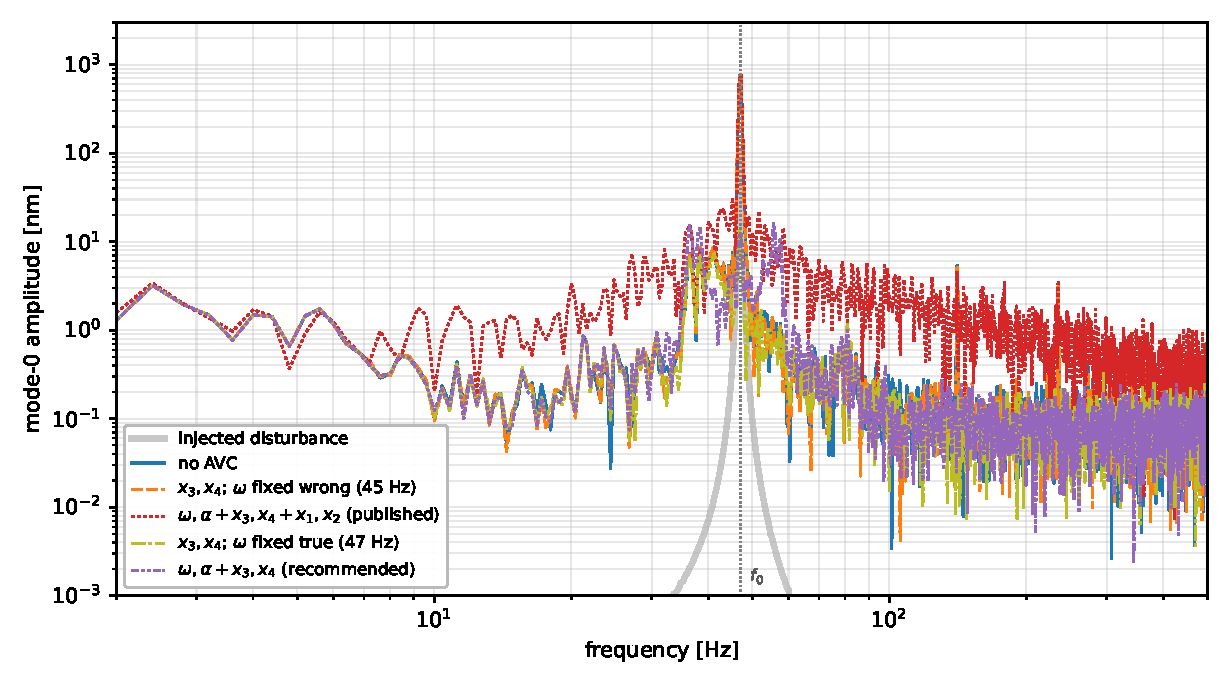
\includegraphics[width=0.7\textwidth]{avc_ablation_psd.pdf}
\caption{Steady-state mode-0 residual spectra, with the injected disturbance for reference (grey).
%
Without AVC the loop amplifies the tone to \SI{17.4}{dB} above the input.
%
The two failing configurations track that peak exactly; the two working ones remove it, ending \SI{18.2}{dB} \emph{below} the input.
%
In the original configuration, adapting both the plant and the disturbance estimate, a broadband amplification is generated at all frequencies due to a wrong phasing of the command.}
\label{fig:psd}
\end{figure}

\section{Analysis: what works, and what cannot}
\label{sec:analysis}

The configuration above deliberately switches off the plant adaption. This section analyzes why.
%

\subsection{What the measurement contains}
\label{sec:contains}

The algorithm models the measured residual as a sinusoid at the tracked
frequency,
%
\begin{equation}
  y(t)=\mathrm{Re}(Z)\cos\alpha(t)+\mathrm{Im}(Z)\sin\alpha(t),
  \qquad
  Z=\vartheta\,\overline{P_\star}+\Lambda_\star
   =\Lambda_\star-\kappa\hat\Lambda,
  \qquad
  \kappa=\overline{\left(\frac{P_\star}{\hat P}\right)} ,
  \label{eq:Z}
\end{equation}
%
with $P_\star,\Lambda_\star$ the true plant and disturbance and $\vartheta$
the applied control.

Once $\alpha(t)$ is known, the measurement depends on the unknown parameters only through the complex number $Z$, i.e.\ through two real numbers.
%
% This is not a statement about sampling rate: at \SI{1}{kHz} a \SI{47}{Hz} tone is sampled about 21 times per period, but those samples are 21 noisy views of the \emph{same} two numbers, not 21 independent constraints on $(P,\Lambda)$.
%
Nor does it improve with observation time.
%
The regressor has the form $\vW=\cos\alpha\,\mathbf{u}_1+\sin\alpha\,\mathbf{u}_2$ with $\mathbf{u}_{1,2}$ independent of phase (Sec.~\ref{sec:pe}), so $\sum_t\vW\vW^\top$ has rank two for any number of samples (length of the experiment).
%
% : over $2\times10^4$ samples, several hundred vibration periods, the eigenvalues are $(118.8,\,118.8,\,7\!\times\!10^{-15},\,-4\!\times\!10^{-15})$.
%
% More data buys precision on those two numbers, never additional rank, and rank is what separating the plant from the disturbance requires.

The whole experiment therefore yields two real numbers about the static parameters, however long it runs.
%
Every identifiability question reduces to asking which parameters are determined by $Z$.

\subsection{Why plant identification is ill-posed}
\label{sec:illposed}

Treat the true $(P_\star,\Lambda_\star)$ as jointly unknown, with the applied command $\vartheta$ known. 
%
Then $Z=\vartheta\overline{P_\star}+\Lambda_\star$ is a {linear} map $\mathbb{R}^4\to\mathbb{R}^2$ both conjugation and multiplication by $\vartheta$ are $\mathbb{R}$-linear, so its kernel is exactly two-dimensional:
%
\begin{equation}
  \delta Z=\vartheta\,\overline{\delta P}+\delta\Lambda=0
  \qquad\Longleftrightarrow\qquad
  \delta\Lambda=-\vartheta\,\overline{\delta P} .
  \label{eq:kernel}
\end{equation}
%
Any change in the plant can be exactly absorbed by a change in the disturbance, leaving every measurement unchanged at every phase, for all time.
%
% The same holds when the varied quantities are the \emph{estimates}
% $(\hat P,\hat\Lambda)$, even though $Z$ is then a nonlinear function of
% them. It depends on the pair only through the emitted command
% $\vartheta=-\hat\Lambda/\overline{\hat P}$, whose level sets
% $\{\hat\Lambda=c\,\overline{\hat P}\}$ are themselves exact
% $\mathbb{R}$-linear planes; each fibre therefore coincides with its own
% tangent space, and the degeneracy is again exact rather than
% infinitesimal. Read this way the unobservable directions are simply those
% along which the algorithm emits the \emph{same command}, so that nothing
% physical changes.
%
% One caveat: the plane in \eqref{eq:kernel} depends on $\vartheta$, hence on
% where the estimate currently sits. It is a field of planes rather than one
% fixed subspace --- integrable, since it is the fibre structure of
% $\vartheta$, so a trajectory drifting along it stays unobservable
% indefinitely.
%
% The two are not separately identifiable, and this is a property of the experiment rather than of the algorithm.

In practice, $\hat P$ drifts along this kernel.
%
It does not merely fail to converge: $\hat P$ sits in the denominator of \eqref{eq:theta}, so the drift feeds back into the control and the loop diverges.
%
In simulation the plant estimate wanders over three decades in magnitude and the full $\pm180^\circ$ in phase.
%
$P$ is however not \emph{needed} as an estimate. Two things follow.
%
%
A cancelling solution exists for any plant estimate. From \eqref{eq:Z}, the plant appears inside the ratio $\kappa$, and setting $Z=0$ gives
%
\begin{equation}
  \hat\Lambda_\infty=\Lambda_\star/\kappa ,
  \label{eq:fixedpoint}
\end{equation}
%
which is well-defined for any $\kappa\neq0$. Perfect cancellation is then {possible} whatever finite non-zero $\hat P$ is used.
%
{Whether the loop reaches that solution}, and what happens to $\hat P$
while it does, is a question about dynamics rather than about
\eqref{eq:Z}. It is treated in Sec.~\ref{sec:conv}.
%
Note already that by \eqref{eq:fixedpoint} a magnitude error in $\hat P$
does not degrade the steady state: it rescales the converged
$\hat\Lambda$ and changes the convergence rate, but still yields $Z=0$.
%
What AVC needs from the plant is a phase, within a generous margin.

\subsection{Cost Function Analysis}
\label{sec:cost}
%
The minimized quantity $J=\tfrac12(\vW^\top\vx-y)^2$ is an \emph{equation error}: it measures whether the model is consistent with itself, not whether the vibration has been cancelled.
%
The model, however, is self-consistent by construction.

Substituting the control law \eqref{eq:thetacomplex},
$\vartheta=-P\Lambda/D$ with $D=|P|^2+\epsilon$, into the prediction gives,
in the notation of \eqref{eq:Z},
\begin{equation}
  \vW^\top\hat\vx
  =\mathrm{Re}(\hat Z)\cos\alpha+\mathrm{Im}(\hat Z)\sin\alpha,
  \qquad
  \hat Z=\vartheta\overline{\hat P}+\hat\Lambda
        =-\frac{|\hat P|^2}{D}\hat\Lambda+\hat\Lambda
        =\hat\Lambda\,\frac{\epsilon}{D}
  \;\xrightarrow[\epsilon\to0]{}\;0 ,
  \label{eq:Zhat}
\end{equation}
Because $\vartheta$ is built to cancel $\hat\Lambda$, the model always predicts perfect cancellation of its own estimate, whatever that estimate is.
%
With the published $\epsilon=0$ the prediction is identically zero, so
\begin{equation}
  J=\tfrac12\big(0-y\big)^2=\tfrac12y^2 ,
\end{equation}
which does not depend on $\vx$ at all.
%
A cost independent of its parameters has zero gradient.
%
Notice that $y$ depends on the estimate through the loop, but the equation error definition does not involve dynamics, so the instantaneous gradient is computed holding $y$ fixed, and $y$ is invariant on the current estimate.

% \paragraph{Constant, not zero.}
% The statement above is easy to misread, so it is worth separating two things.
% %
% The cost $J$ is \emph{not} zero: it equals $\tfrac12y^2$, which for a typical residual is large.
% %
% Neither is the error $e$, which equals $-y$.
% %
% What is identically zero is the \emph{prediction term} $\vW^\top\hat\vx$, and the consequence is that $J$ takes the \emph{same} large value for every estimate.
% %
% Numerically, fixing $y=137.4$ and evaluating $J$ at five very different
% estimates (plant components spanning $\pm5$, disturbance components
% $\pm90$) gives $\vW^\top\hat\vx\sim10^{-15}$ and $J=9439.3800$ in every
% case, identical to four decimals.
% %
% The cost is large; it simply does not \emph{move} when the parameters move, which is what makes it useless to descend.
% %
% With $\epsilon=10^{-2}$ the same test gives $J$ between $9437.99$ and $9447.65$, a $0.1\%$ wiggle: that is the entire parameter dependence available to the exact gradient.

% \paragraph{Why $y$ may be treated as data.}
% One might object that $y$ surely depends on the estimate, since the residual is the outcome of the correction the estimate produced.
% %
% It does, but on \emph{past} estimates, through the loop.
% %
% With at least one frame of delay between command and measurement, $\partial y(t)/\partial\hat\vx(t)=0$, so holding $y$ fixed in the instantaneous gradient is legitimate.

% That is precisely the indictment.
% %
% The cost contains no dynamics: no plant, no delay, no time.
% %
% The only parameter dependence it can express is the instantaneous algebraic one, and that one is identically zero.
% %
% The dependence that matters, from past parameters through the applied command to the present residual, is invisible to it.
% %
% The gradient computation is correct; the objective is inert.
The update \eqref{eq:update} is therefore not a gradient descent on the cost it nominally minimizes.
%
Holding $\vW$ fixed while differentiating is the defining step of the classical \emph{equation-error} or \emph{pseudo-linear regression} family: if $\vW$ really were independent of $\vx$, then $\vW e$ \emph{is} the exact gradient and \eqref{eq:update} is textbook LMS~\cite{haykin2013}, with its convergence theory.
%
% The same device appears in Feintuch's algorithm~\cite{feintuch1976} for recursive (IIR) adaptive filters, where the parameter dependence of the regressor is likewise ignored;
%
% it was pointed out soon afterwards that the result is not a gradient method~\cite{widrow1977comments} and can converge to biased solutions~\cite{shynk1989}, which is why filtered-X schemes~\cite{morgan1980,kuo1996} filter the regressor through an estimate of the secondary path instead.
%
The algorithm can be justified by analyzing the dynamics it generates, not by appealing to the cost it minimizes, through \eqref{eq:integral} below, and the stability proofs cited by the paper~\cite{pigg2010tcst,pigg2010cdc}.
%
%
% The ``gradient descent on $\varepsilon^2$'' framing is a post-hoc rationalization, and the distinction is not academic: it is exactly why computing the gradient \emph{more accurately} makes the algorithm worse rather than better.
Since $e\simeq-y$, the disturbance part of \eqref{eq:update} becomes, after
averaging over a cycle,
%
\begin{equation}
  \dot{\hat\Lambda}\;\propto\;Z\;=\;\Lambda_\star-\kappa\hat\Lambda ,
  \label{eq:integral}
\end{equation}
%
a first-order integral controller on the residual.
%
What makes the algorithm effective is therefore integral action on the
measured residual, which is a control objective, rather than the
minimization of \eqref{eq:Zhat}.

A corollary: $\hat\Lambda$ converges to the command that cancels the disturbance, not to the disturbance itself.
%
Across runs with different frozen $\hat P$ the converged $|\hat\Lambda|$ scales with $|\hat P|$ to about $1\%$, as $\hat\Lambda_\infty=\Lambda_\star/\kappa$ requires, while all of them cancel equally well.
%
It is a controller state, not an estimate.

\subsection{Convergence analysis}
\label{sec:conv}

The two halves of the state converge in different ways. 
%
Equation~\eqref{eq:update} applied to \eqref{eq:W}, with the plant half carrying its own gain $c_x$ (Sec.~\ref{sec:params}), reads
%
\begin{equation}
\begin{aligned}
  x_1 &\leftarrow x_1-\mu\,c_x\,(\theta_c c+\theta_s s)\,e, &\qquad
  x_3 &\leftarrow x_3-\mu\,c\,e,\\
  x_2 &\leftarrow x_2-\mu\,c_x\,(\theta_s c-\theta_c s)\,e, &\qquad
  x_4 &\leftarrow x_4-\mu\,s\,e .
\end{aligned}
\label{eq:components}
\end{equation}

Grouping as in Sec.~\ref{sec:alg}, $\hat P=x_1+ix_2$ and
$\hat\Lambda=x_3+ix_4$, the right-hand pair gives
$\delta x_3+i\,\delta x_4=-\mu(c+is)e$, and the left-hand pair uses the
identity $W_1+iW_2=\vartheta e^{-i\alpha}$. Hence
%
\begin{equation}
  \delta\hat\Lambda=-\mu\,e^{\,i\alpha}\,e ,
  \qquad\qquad
  \delta\hat P=-\mu\,c_x\,\vartheta\,e^{-i\alpha}\,e .
  \label{eq:twoincrements}
\end{equation}
%
The two are identical except for the gain $c_x$ and the factor $\vartheta e^{-2i\alpha}$.
%
The measured residual can be written equivalently as
%
\begin{equation}
  y(t)=\mathrm{Re}(Z)\cos\alpha+\mathrm{Im}(Z)\sin\alpha
      =\mathrm{Re}\!\left(Z\,e^{-i\alpha}\right) ,
  \label{eq:yforms}
\end{equation}
%
Recall also $e\simeq-y$, since the prediction term is $\mathcal{O}(\epsilon)$ by \eqref{eq:Zhat}.
%
Substituting \eqref{eq:yforms} into \eqref{eq:twoincrements} and averaging over one cycle, using $\langle e^{\pm2i\alpha}\rangle=0$:
%
\begin{equation}
  \big\langle e^{\,i\alpha}y\big\rangle=\tfrac12 Z ,
  \qquad
  \big\langle e^{-i\alpha}y\big\rangle=\tfrac12\overline{Z} ,
  \qquad\Longrightarrow\qquad
  \dot{\hat\Lambda}=\gamma Z ,
  \quad
  \dot{\hat P}=\gamma_p\,\vartheta\,\overline{Z} ,
  \label{eq:twohalves}
\end{equation}
%
with $\gamma,\gamma_p>0$.

% \paragraph{Why average at all.}
% That step deserves justification, because it is the one place where an
% approximation enters an otherwise exact chain.
% %
% Substituting \eqref{eq:yforms} into \eqref{eq:twoincrements} \emph{without}
% averaging, and using $\mathrm{Re}(Ze^{-i\alpha})=\tfrac12(Ze^{-i\alpha}+\overline{Z}e^{i\alpha})$, the increment of the disturbance state at sample $k$ is exactly
% %
% \begin{equation}
%   \hat\Lambda_{k+1}-\hat\Lambda_k
%   =\mu\,e^{i\alpha_k}y_k
%   =\underbrace{\tfrac12\mu\,Z_k}_{\text{secular}}
%   \;+\;\underbrace{\tfrac12\mu\,\overline{Z_k}\,e^{2i\alpha_k}}_{\text{counter-rotating}} ,
%   \qquad \alpha_k=\alpha_0+k\omega T_s .
%   \label{eq:exactincrement}
% \end{equation}
% %
% Two features of \eqref{eq:exactincrement} block a direct eigenvalue analysis.
% It is \emph{periodically time-varying}, through $e^{2i\alpha_k}$, so it has no
% constant coefficients and no fixed point in the ordinary sense; and it is
% \emph{real}-linear rather than complex-linear, because $\overline{Z}$ appears
% alongside $Z$. Averaging removes both obstructions at once.

% The two terms behave completely differently over a cycle. Summing
% \eqref{eq:exactincrement} over the $N=1/(f_{\mathrm{vib}}T_s)$ samples of one
% period, during which $\hat\Lambda$ --- and therefore $Z$ --- changes by only
% $O(\mu N)$ and may be treated as frozen:
% %
% \begin{equation}
%   \hat\Lambda_{k+N}-\hat\Lambda_k
%   \;\simeq\;
%   \tfrac12\mu N\,Z_k
%   \;+\;\tfrac12\mu\,\overline{Z_k}\,e^{2i\alpha_k}
%        \underbrace{\frac{e^{2i\omega NT_s}-1}{e^{2i\omega T_s}-1}}_{=\;0} .
%   \label{eq:onecycle}
% \end{equation}
% %
% The first term accumulates coherently, $N$ steps all pushing the same way ---
% this is the integral action. The second is a geometric series whose ratio
% completes two full turns per period, $\omega NT_s=2\pi$, so it sums to
% \emph{exactly} zero; away from an integer number of cycles it is not zero but
% it is bounded by $\tfrac12\mu|Z|/|\sin\omega T_s|$, an oscillation rather than
% an accumulation. Dividing \eqref{eq:onecycle} by the period $NT_s$ gives
% \eqref{eq:twohalves} with $\gamma=\mu/(2T_s)=g_x/2$.

Averaging is an approximation, and the error of such approximation is known: the averaged solution departs from the exact recursion by $O(\mu)$ on timescales $O(1/\mu)$~\cite{sanders2007,khalil2002}, the small parameter being the
per-sample step $\mu=g_xT_s$. Figure~\ref{fig:averaging} confirms both the size ($0.5\%$ of $|\hat\Lambda_\infty|$ at $g_x=3$) and the linear scaling.
%
What licenses the stability analysis that follows is the second half of the averaging theorem, stating that hyperbolic equilibria of the averaged system are hyperbolic periodic orbits of the exact one, with the same stability type.
%
\begin{figure}
\centering
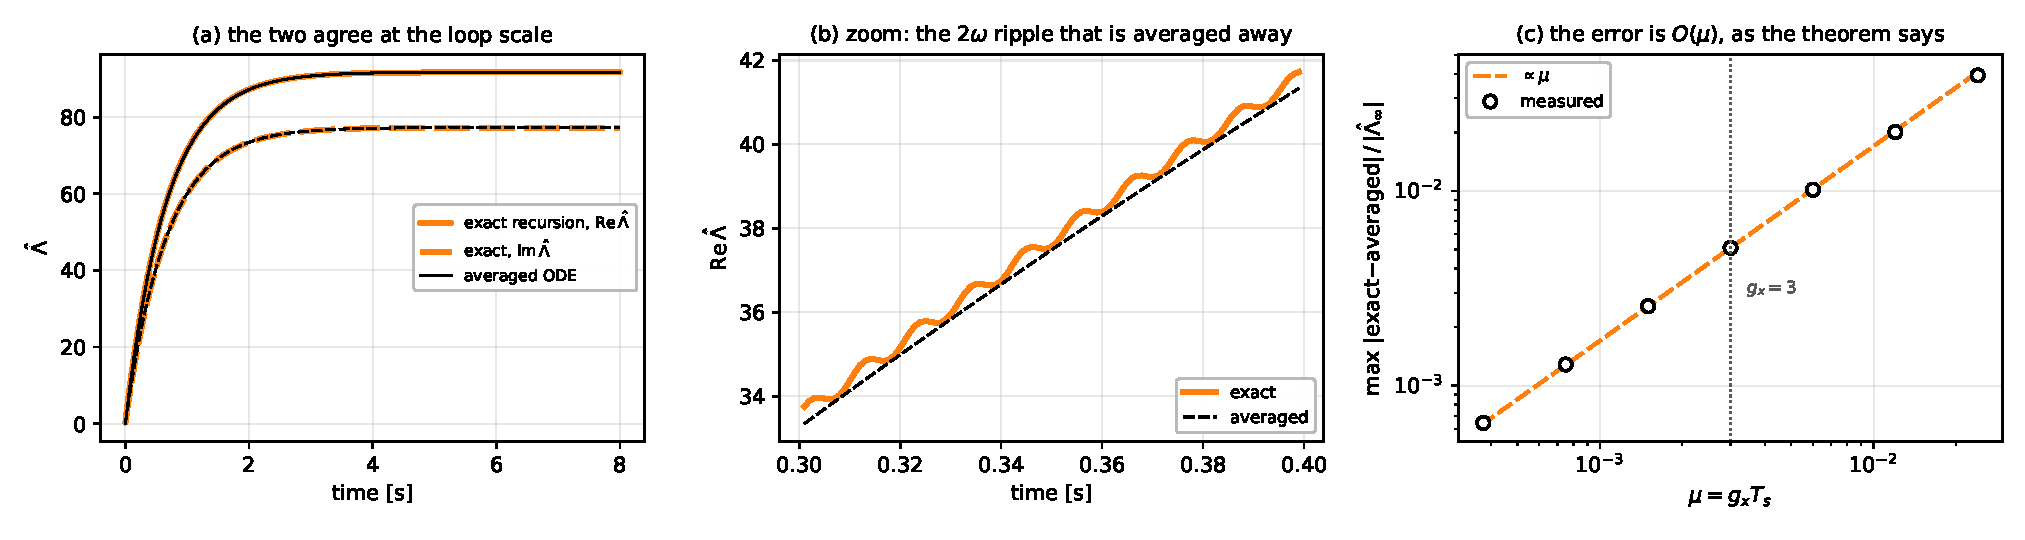
\includegraphics[width=\textwidth]{avc_averaging.pdf}
\caption{The averaging step. (a) Exact per-sample recursion against the
solution of the averaged ODE \eqref{eq:twohalves}, at $g_x=3$. (b) Zoom: the
$2\omega$ ripple that the average removes. (c) Maximum discrepancy against the
small parameter $\mu=g_xT_s$, confirming the $O(\mu)$ error bound.}
\label{fig:averaging}
\end{figure}
%
So, $\hat\Lambda$ integrates the residual, while $\hat P$ has a nonlinear dynamics lead by
%
\begin{equation}
  \vartheta=-\frac{\hat\Lambda}{\overline{\hat P}}.
  \notag
\end{equation}
%
We can study dynamic convergence of the two dynamical subsystems. Starting from $\Lambda$, we can expand as follows
\begin{equation}
  \dot{\hat{\Lambda}} = \gamma \left(\vartheta \overline{P_\star} + \Lambda_\star\right). 
\end{equation}
Recalling the definition of $\vartheta$, we can write
\begin{equation}
  \dot{\hat{\Lambda}} = \gamma \left(-\frac{\hat{\Lambda}}{\overline{\hat{P}}} \overline{P_\star} + \Lambda_\star\right) = -\gamma \frac{\overline{P_\star}}{\overline{\hat{P}}} \hat{\Lambda} + \gamma \Lambda_\star.
  \label{eq:lambda_dynamics}
\end{equation}
This is an integrator dynamics. Introducing the complex loop gain
%
\begin{equation}
  \kappa \;=\; \frac{\overline{P_\star}}{\overline{\hat P}}
          \;=\; \overline{\left(\frac{P_\star}{\hat P}\right)} ,
  \label{eq:kappa}
\end{equation}
%
equation \eqref{eq:lambda_dynamics} becomes
$\dot{\hat\Lambda}=-\gamma\kappa\,(\hat\Lambda-\hat\Lambda_\infty)$ with the
fixed point
%
\begin{equation}
  \hat\Lambda_\infty=\frac{\Lambda_\star}{\kappa}
                    =\frac{\overline{\hat P}}{\overline{P_\star}}\Lambda_\star .
  \label{eq:laminf}
\end{equation}
%
This is a {complex} linear system with the single eigenvalue $-\gamma\kappa$, so the error $\delta=\hat\Lambda-\hat\Lambda_\infty$ evolves as $\delta(t)=e^{-\gamma\kappa t}\delta(0)$, i.e.\ (the factor $\tfrac12$ in \eqref{eq:twohalves} fixing $\gamma=g_x/2$)
%
\begin{equation}
  |\delta(t)|=e^{-\gamma\,\mathrm{Re}\kappa\,t}\,|\delta(0)| ,
  \label{eq:deltadecay}
\end{equation}
%
Convergence therefore requires $\mathrm{Re}\,\kappa>0$, which by \eqref{eq:kappa} is a condition on the plant {phase} alone:
%
\begin{equation}
  \big|\arg P_\star-\arg\hat P\big|<90^\circ.
  \label{eq:margin}
\end{equation}
%
In continuous time a plant {magnitude} error of a factor ten is harmless and only slows convergence, whereas a phase error of $91^\circ$ causes instability.
%
Figure~\ref{fig:margin} shows this results through the SPECULA simulation.
%
The component-wise update \eqref{eq:components} is run with the plant half frozen at $\hat P=|P_\star|e^{i(\arg P_\star+\Delta\varphi)}$, so that $|\kappa|=1$ and the phase error is the only variable, on a single noiseless vibration.
%
% The measured exponential rate follows $\tfrac12 g_x\cos\Delta\varphi$ to three or four digits over the whole range and changes sign exactly at $\Delta\varphi=90^\circ$: at $89^\circ$ the disturbance error still decays, at $91^\circ$ it grows without bound.
%
\begin{figure}
\centering
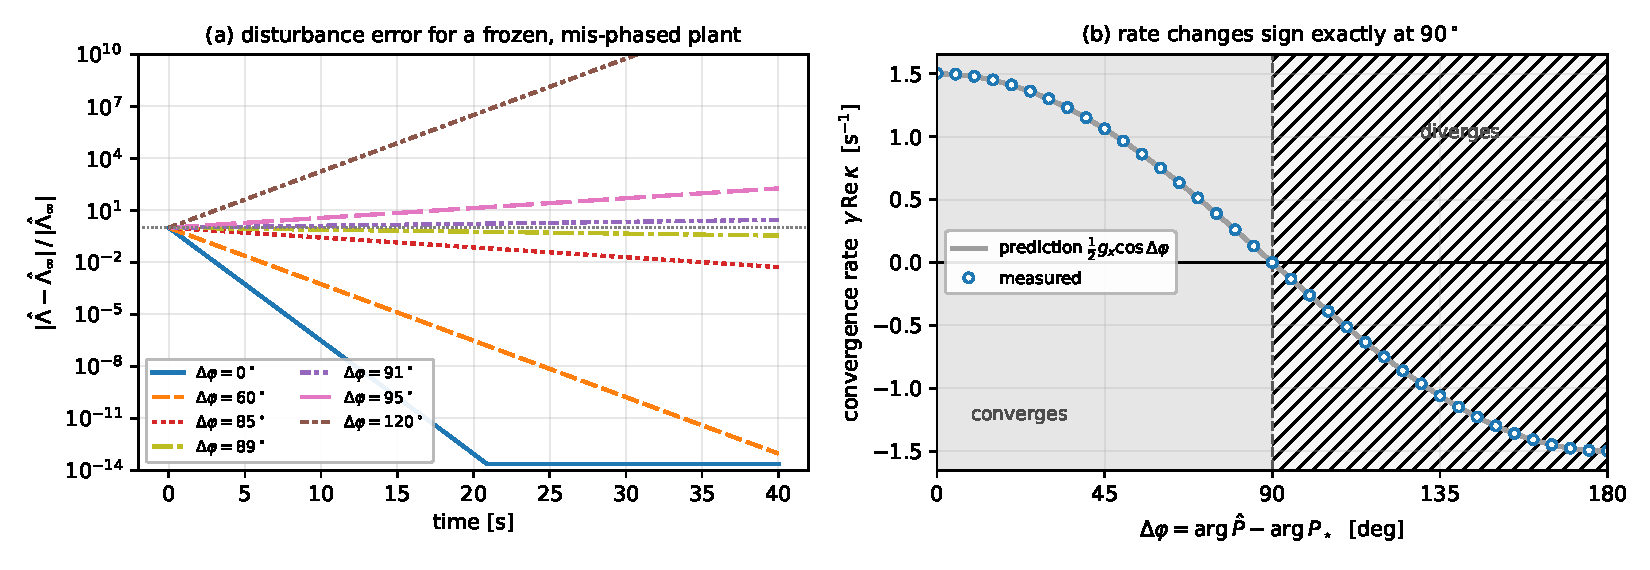
\includegraphics[width=\textwidth]{avc_margin_check.pdf}
\caption{Violation of the margin condition \eqref{eq:margin}, with the plant
estimate frozen at a controlled phase error $\Delta\varphi$ and $|\kappa|=1$.
(a) Normalised disturbance error $|\hat\Lambda-\hat\Lambda_\infty|$:
exponential decay for $\Delta\varphi<90^\circ$ (solid), exponential growth
for $\Delta\varphi>90^\circ$ (dashed); (b) Measured rate against the prediction
$\gamma\,\mathrm{Re}\,\kappa=\tfrac12 g_x\cos\Delta\varphi$.}
\label{fig:margin}
\end{figure}

In discrete time the magnitude does re-enter the stability condition. The exact one-sample increment is $\delta\hat\Lambda=-\tfrac12\mu\big(\kappa\delta+\overline{\kappa}\,\overline{\delta}\,e^{2i\alpha}\big)$ with $\mu=g_xT_s$ as in \eqref{eq:update}. The stability limit is set by the worst phase of the cycle, at which the two terms align and the sample gain becomes $1-\mu\kappa$. Requiring that to lie in the unit disk gives
%
\begin{equation}
  \mu<\frac{2\,\mathrm{Re}\,\kappa}{|\kappa|^{2}}.
  \label{eq:stepbound}
\end{equation}
%
% which a direct sweep of $g_x$ to divergence reproduces to four digits for real
% $\kappa$ ($\mu_{\mathrm{thr}}=2.0007$ against $2$ for $\kappa=1$, $4.0014$
% against $4$ for $\kappa=1/2$). The bound is nowhere near binding in practice:
% the calibrated loop has $\kappa\simeq1$, hence $g_x<2000$ against the $g_x=3$
% actually used. It is the phase condition \eqref{eq:margin}, not the step size,
% that constrains the algorithm.
% %
It is worth noting that the limit is $\hat\Lambda_\infty\neq\Lambda_\star$ unless $\hat P=P_\star$. What $\hat\Lambda$ converges to is whatever value cancels the tone \emph{given} the plant estimate in use, since $\vartheta_\infty=-\hat\Lambda_\infty/\overline{\hat P} =-\Lambda_\star/\overline{P_\star}=\vartheta_\star$.
%
The disturbance is not identified, but the canceling {command} is. For the control problem that is sufficient, and it is why an approximate calibration of $\hat P$ still gives full rejection (Sec.~\ref{sec:best}).
%
Notice that the convergence of the $\hat{\Lambda}$ dynamics implies convergence of the plant estimate $\hat{P}$ dynamics, since $\vartheta$ converges to $\vartheta_\star$ and $Z$ converges to zero. However, the plant estimate $\hat{P}$ does not converge to the true plant $P_\star$, but rather drifts along a manifold of equivalent solutions that yield the same control action. 
%
Also, existence of a stationary point does not guarantee stability. The problem of the neutral stability of the plant estimate is that, if the plant estimate drifts too far from the true plant, the convergence condition \eqref{eq:margin} may be violated, leading to divergence of the disturbance estimate and ultimately to instability of the control loop.
% The above holds for a fixed $\hat P$. Turning to the plant equation of
% \eqref{eq:twohalves}, the first observation is that it shares its driving
% term with the disturbance equation: both increments are proportional to
% $Z$. Hence $Z=0$ switches off \emph{both} simultaneously, and the plant
% half has no stationarity condition of its own --- it stops because the
% signal driving it has vanished, not because it has arrived anywhere. Nor is
% there any notion of $\hat P$ converging separately: if $\hat\Lambda$ is
% still moving then $Z\neq0$ and $\hat P$ is moving too.

% That the two halves are not competing is seen by differentiating
% $\vartheta=-\hat\Lambda/\overline{\hat P}$ and substituting
% \eqref{eq:twohalves}, which gives exactly
% %
% \begin{equation}
%   \dot\vartheta=-\big(\gamma+\gamma_p|\vartheta|^2\big)
%                 \frac{Z}{\overline{\hat P}} ,
%   \qquad
%   Z=\vartheta\,\overline{P_\star}+\Lambda_\star .
%   \label{eq:thetadyn}
% \end{equation}
% %
% Both halves push the command in the same direction, and \eqref{eq:thetadyn}
% has the single fixed point $\vartheta_\star$, stable under the same
% condition $\mathrm{Re}\,\kappa>0$. So the quantity that genuinely converges
% is $\vartheta$, two real numbers, while the algorithm carries four. Two of
% those four are redundant, and the redundancy is exactly the set
% %
% \begin{equation}
%   \mathcal{M}=\{\vartheta=\vartheta_\star\}
%    =\{\hat\Lambda=-\vartheta_\star\overline{\hat P}\} ,
%   \label{eq:eqmanifold}
% \end{equation}
% %
% a two-dimensional surface of equilibria parameterized freely by $\hat P$:
% every plant estimate has a matching $\hat\Lambda$ that cancels the tone,
% and the algorithm is equally content with all of them.

% Linearizing \eqref{eq:twohalves} at a point of $\mathcal{M}$ confirms this.
% Two of the four eigenvalues are exactly zero, and \emph{their eigenvectors
% span the tangent plane of} $\mathcal{M}$ --- the directions along which the
% state can move with no restoring force whatsoever. The other two are
% transverse to $\mathcal{M}$ and carry the dynamics \eqref{eq:thetadyn}:
% numerically their real part follows $-C\cos\Delta\varphi$ with
% $\Delta\varphi=\arg\hat P-\arg P_\star$, changing sign exactly at
% $90^\circ$ ($-87.3$ at $\Delta\varphi=85^\circ$, $+87.3$ at $95^\circ$).
% With $\hat P$ frozen, by contrast, $\hat\Lambda\mapsto\vartheta$ is a
% bijection: the two zero eigenvalues disappear, $\mathcal{M}$ collapses to
% the isolated point \eqref{eq:fixedpoint}, and the equilibrium is hyperbolic
% and exponentially stable.

% \paragraph{Why neutral stability is not benign.}
% A zero eigenvalue is often dismissed as harmless --- the state simply fails
% to move. That is true only in the noiseless case. In a real loop the
% averaging $\langle e^{i\alpha}y\rangle$ demodulates the \emph{whole}
% residual, not an isolated tone: turbulence and detector noise have power at
% the vibration frequency, so the effective driving term is $Z+n(t)$ with
% $n$ permanently non-zero. A direction with a negative eigenvalue absorbs
% that as bounded jitter. A direction with a \emph{zero} eigenvalue
% integrates it, and integrated noise is a random walk, which has no
% stationary distribution. So $\hat P$ does not settle anywhere; it wanders,
% without bound, along $\mathcal{M}$.

% The wandering would still be tolerable if $\mathcal{M}$ were attracting
% everywhere. It is not: by \eqref{eq:margin} the transverse directions are
% stable only inside a cone of half-angle $90^\circ$ about $\arg P_\star$,
% and the coordinate that decides membership of that cone --- $\arg\hat P$ ---
% is precisely the one performing the random walk. The mechanism is therefore
% self-defeating: the unconstrained drift eventually carries the phase out of
% the cone, the transverse eigenvalues change sign, $\vartheta$ is pushed
% \emph{away} from $\vartheta_\star$, and $Z$ grows instead of decaying. The
% disturbance integrator, still working faithfully, then integrates a signal
% that never dies and ramps without bound. This is the divergence of
% Sec.~\ref{sec:expconf}: not the $1/|\hat P|^2$ singularity by itself, but
% free drift along a surface whose transverse stability depends on where on
% the surface one happens to be.

% Figure~\ref{fig:wander} shows this in the simulation. With the plant
% adapted, $\arg\hat P$ makes $204$ complete turns in \SI{10}{s} and spends
% only $47\%$ of the time inside the stability cone; $|\hat\Lambda|$ ramps
% linearly (increments of $2580$, $2577$, $2598$, $2629$ over successive
% \SI{2}{s} windows --- a straight line to $1\%$), and the mode-0 residual is
% \SI{644}{nm} RMS against \SI{630}{nm} for the loop without AVC at all,
% i.e.\ no rejection whatsoever. Freezing the plant at the calibrated value
% leaves $\hat\Lambda$ settling at $1420$ and the residual at \SI{28}{nm}.

% \begin{figure}[t]
% \centering
% 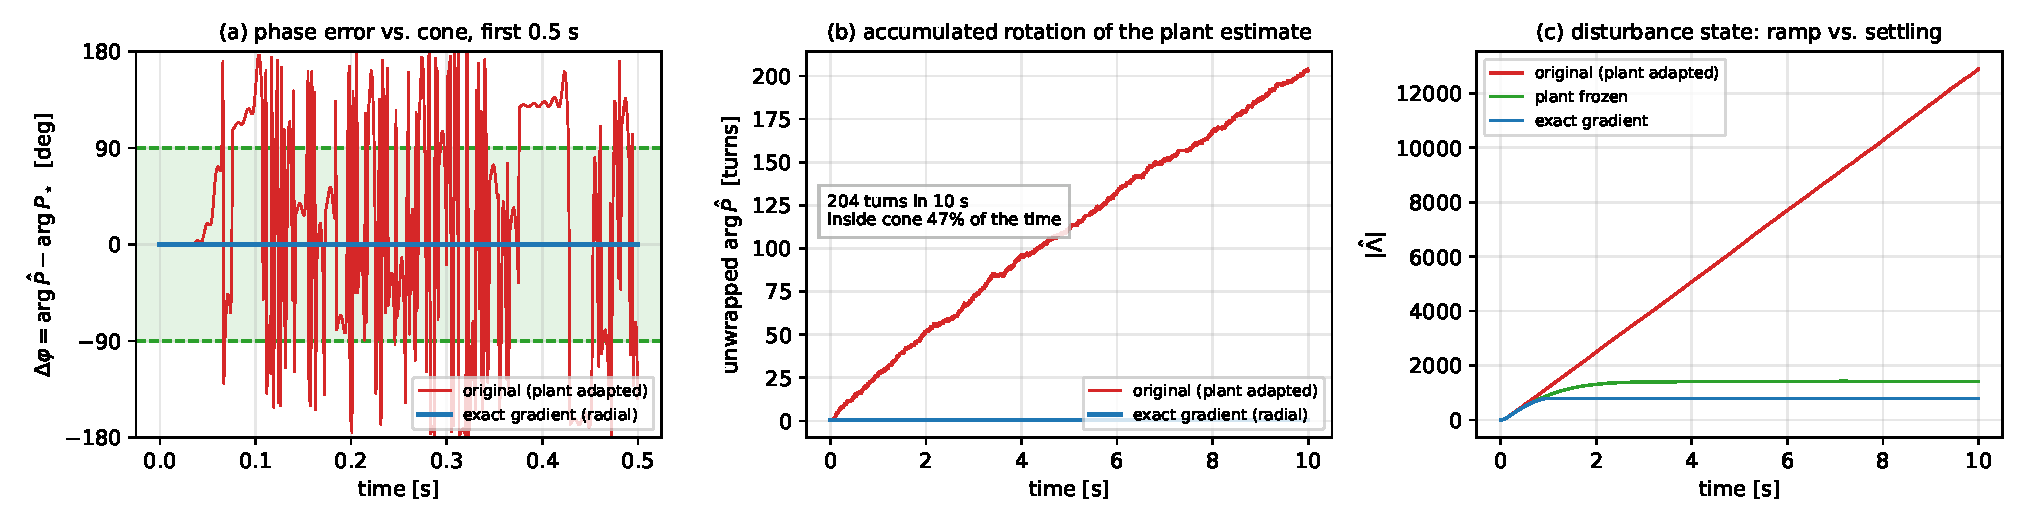
\includegraphics[width=\textwidth]{avc_phase_wander.pdf}
% \caption{Drift of the plant estimate along $\mathcal{M}$.
% (a) Phase error $\Delta\varphi=\arg\hat P-\arg P_\star$ over the first
% \SI{0.5}{s}; the shaded band is the stability cone \eqref{eq:margin}.
% (b) Unwrapped $\arg\hat P$ over the whole run: the original update
% accumulates $204$ turns, the exact-gradient variant exactly none.
% (c) Consequence on the disturbance state: an unbounded ramp when the plant
% is adapted, settling when it is frozen or updated radially.}
% \label{fig:wander}
% \end{figure}

% \paragraph{Why the exact gradient escapes this.}
% The closed form of the exact plant gradient is radial,
% %
% \begin{equation}
%   g_1+ig_2=-2\,\mathrm{Re}\!\left(\frac{\epsilon}{D^{2}}\right)\hat P ,
%   \label{eq:radial}
% \end{equation}
% %
% i.e.\ parallel to $\hat P$ itself. It can rescale the plant estimate but
% can never rotate it. The variant is thus \emph{structurally incapable} of
% leaving the stability cone: the blue trace in Fig.~\ref{fig:wander}(b) is
% flat to $0.00^\circ$ over $10^4$ steps while $|\hat P|$ moves freely
% between $3.6$ and $7.2$. It does not identify the plant any better than the
% original --- it still has a zero direction, now in $|\hat P|$ --- but its
% zero direction is the harmless one, $|\kappa|$ being absent from
% \eqref{eq:margin}. That, rather than any improvement in identification, is
% why the hybrid configuration is stable.

% All of this is the classical picture for an adaptive system without
% persistent excitation~\cite{ljung1999,sastry1989}: the output error
% converges, the parameters need not. The practical conclusion is that the
% two zero eigenvalues must be removed by construction --- by freezing
% $\hat P$, or at least by confining its update to the phase-preserving
% direction --- which is the justification for the configuration of
% Sec.~\ref{sec:best}.

\subsection{Are the regressors persistently exciting?}
\label{sec:pe}

This is the classical way in system identification theory to phrase the analysis.
%
Persistent excitation requires the averaged information matrix $\langle\vW\vW^\top\rangle$ to be positive definite.
%
Writing
$\vW=c\,\mathbf{u}_1+s\,\mathbf{u}_2$ with
$\mathbf{u}_1=(\theta_c,\theta_s,1,0)^\top$ and
$\mathbf{u}_2=(\theta_s,-\theta_c,0,1)^\top$, and averaging over a cycle
($\langle c^2\rangle=\langle s^2\rangle=\tfrac12$, $\langle cs\rangle=0$),
%
\begin{equation}
  \langle\vW\vW^\top\rangle
  =\tfrac12\big(\mathbf{u}_1\mathbf{u}_1^\top+\mathbf{u}_2\mathbf{u}_2^\top\big)
  =\tfrac12\big(|\vartheta|^2+1\big)\,\Pi ,
  \label{eq:info}
\end{equation}
%
with $\Pi$ the projector onto $\mathrm{span}\{\mathbf{u}_1,\mathbf{u}_2\}$.
%
The spectrum is $\{\lambda,\lambda,0,0\}$ with $\lambda=\tfrac12(|\vartheta|^2+1)$, the information matrix is of rank 2, and the regressors are not persistently exciting of order 4.

This is the textbook statement that \textbf{a single sinusoid is persistently exciting of order 2}~\cite{ljung1999,sastry1989}.
%
It supports the estimation of exactly two parameters; four would require excitation of order 4, that is at least two distinct frequencies.
%
% The algorithm asks a one-tone experiment for four numbers, and the two it cannot deliver are precisely the plant components.
%
It is worth stressing that \eqref{eq:info} is not a consequence of the
particular $\vW$ of \eqref{eq:W}: \emph{no} choice of four regressors can
do better, as long as the model output is a single tone.
% Suppose the model
% is $y=\vW^\top\vx$ with $y$ a sinusoid at one frequency. Setting
% $\vx=\mathbf{e}_i$ shows that each component $W_i(t)$ must itself be a
% realizable output, i.e.\ a combination of $\cos\alpha$ and $\sin\alpha$.
% Hence
% %
% \begin{equation}
%   \vW(t)=\cos\alpha(t)\,\mathbf{a}+\sin\alpha(t)\,\mathbf{b}
% \end{equation}
% %
% for \emph{fixed} vectors $\mathbf{a},\mathbf{b}\in\mathbb{R}^4$, whatever
% the parameterization, so $\vW$ is confined to
% $\mathrm{span}\{\mathbf{a},\mathbf{b}\}$ and
% $\langle\vW\vW^\top\rangle$ has rank at most two.
% %
% We verified this on several unrelated four-parameter single-tone models
% (the AVC regressor, arbitrary $\cos/\sin$ mixtures, and random ones): all
% give exactly two non-zero eigenvalues, while adding a second, distinct
% frequency immediately gives rank four.

% The rank-2 limit is therefore a property of the \emph{experiment} --- one
% tone, one applied command --- and not of the algebra chosen to describe it.
% It is the same statement as Sec.~\ref{sec:contains} seen from the parameter
% side: the two dimensions available are exactly $\mathrm{Re}\,Z$ and
% $\mathrm{Im}\,Z$, and no re-parameterization manufactures a third.

% Note also that \eqref{eq:info} is where the factor $(|\vartheta|^2+1)$ of Sec.~\ref{sec:params} comes from: it is the curvature seen by the plant half of the state, and it grows as the correction builds up, which is why that half needs its own gain $c_x$.

% Two remarks.
% %
% Enriching the \emph{disturbance} does not help: modulating its amplitude or phase leaves the two null eigenvalues at $\sim\!10^{-5}$ relative, five orders below the observable pair.
% %
% And the regressor is worse than merely underexciting, because it is \emph{state-dependent}: $\vW$ is built from $\vartheta$, which is slaved to the estimate through \eqref{eq:theta}.
% %
% There is no external reference to enrich; the excitation available to the estimator is generated by the estimator itself, and it stops varying exactly as the algorithm converges.
% %
% Observability has to come from the command side, which is what the offline probe measurement of Sec.~\ref{sec:sim} does.

% \subsection{The frequency loop is the exception}

% Frequency tracking converged in every tested configuration, including those where the plant estimate diverged and cancellation failed entirely.
% %
% The reason is structural.

% A frequency error does not change the \emph{value} of $Z$ within a cycle; it makes $Z$ \emph{rotate} from cycle to cycle at rate $\omega_\star-\hat\omega$.
% %
% That rotation lies in the observable projection, not in the kernel \eqref{eq:kernel}.
% %
% Equivalently: frequency is a property of the observed signal, recoverable
% from the output alone, whereas the plant is a property of an input--output
% map that is never independently excited.
% %
% The PLL is also structurally different from \eqref{eq:update}: it is driven
% by $\sin\alpha\cdot e$ against an \emph{exogenous} reference generated by
% the internal oscillator, so it escapes the self-referential collapse of
% Sec.~\ref{sec:cost}.

% Frequency adaptation is not only possible but necessary.
% %
% The pair $(x_3,x_4)$ integrating in the frame rotating at $\alpha$ is a resonant controller whose loop gain is concentrated at $\hat\omega$, an instance of the internal model principle~\cite{francis1976}; detune it and the correction collapses.

\subsection{Experimental confirmation}
\label{sec:expconf}

Table~\ref{tab:abl} tests these conclusions by ablating which parameters are adapted.
%
All configurations share the loop, the atmosphere and the vibration; only the AVC settings differ.

\begin{table}
\centering\small
\begin{tabular}{lrrrr}
\toprule
adapted parameters & mode-0 RMS & \SI{47}{Hz} amp. & vs.\ baseline & PSD vs.\ input\\
\midrule
none (no AVC)                                        & \SI{629.8}{nm} & \SI{890.3}{nm} & ---        & $+17.4$\,dB\\
$x_3,x_4$; $\omega$ fixed \emph{wrong} (\SI{45}{Hz}) & \SI{646.2}{nm} & \SI{913.6}{nm} & $+0.2$\,dB & $+17.6$\,dB\\
$\omega,\alpha+x_3,x_4+x_1,x_2$ (as published)       & \SI{634.8}{nm} & \SI{892.6}{nm} & $+0.0$\,dB & $+17.4$\,dB\\
$x_3,x_4$; $\omega$ fixed \emph{true} (\SI{47}{Hz})  & \SI{20.7}{nm}  & \SI{16.7}{nm}  & $-34.5$\,dB & $-16.1$\,dB\\
$\boldsymbol{\omega,\alpha+x_3,x_4}$ (recommended)   & \textbf{\SI{26.1}{nm}} & \textbf{\SI{12.1}{nm}} & $\mathbf{-37.4}$\,dB & $\mathbf{-18.2}$\,dB\\
\bottomrule
\end{tabular}
\caption{Ablation over the adapted parameter set.}
\label{tab:abl}
\end{table}


% The two failure modes are not equivalent.
%
% Mistuning the frequency renders the module inert: its spectrum is indistinguishable from the baseline.
% %
% Adapting the plant leaves the vibration untouched \emph{and} raises the broadband floor by one to two decades, which is strictly worse than doing nothing.

\section{A simplified and formally sound AVC algorithm}
\label{sec:simplified}

The analysis of Sec.~\ref{sec:analysis} justifies the formulation of a simpler algorithm that removes the plant adaptation and the optimization approach, based on the ill-posed cost function. The algorithm is a PLL for the vibration frequency and phase and an integrator on the measured residual, with a fixed map from the integrator to the control quadratures, given by the off-line calibration.
%
Because the computation of the control quadratures is not related to $x_1$ and $x_2$ anymore, the safeguards on the plant estimate are not needed, so $\epsilon = 0$ and $\theta_{\min} = 0$
%
What is left is simpler than the original algorithm, performs identically (under suitable operating conditions), and admits a complete stability statement.

\subsection{What is removed}

\paragraph{The plant adaptation.}
The states $x_1,x_2$ are unobservable from a single tone (Sec.~\ref{sec:illposed}), contribute two zero eigenvalues to the closed loop (Sec.~\ref{sec:conv}), and under noise perform an unbounded random walk that may eventually carry $\arg\hat P$ out of the stability cone \eqref{eq:margin}.
%
They are replaced by the closed-loop measurement of Sec.~\ref{sec:calib}, performed once, offline.

\paragraph{The regulariser and the division guard.}
With $\hat P$ fixed, the denominator $|\hat P|^2$ is a calibration constant rather than a state.
%
It cannot approach zero, so $\epsilon$, the clamp threshold $\theta_{\min}$ and the chattering it caused all disappear.
%
In fact no division is performed at run time at all: the map from $(x_3,x_4)$ to the control quadratures is a fixed $2\times2$ matrix, evaluated once at configuration time.

\paragraph{The cost function.}
Section~\ref{sec:cost} shows that $J=\tfrac12 e^2$ is independent of the state it is supposed to minimise.
%
Setting $\epsilon=0$ makes this exact: the prediction term vanishes identically,
%
\begin{equation}
  \vW^\top\vx\equiv0
  \qquad\Longrightarrow\qquad
  e=-y ,
  \label{eq:eisy}
\end{equation}
%
verified to $10^{-14}$ over $2\times10^{4}$ random states.
%
There is therefore nothing to be gained by presenting the update as a gradient step.
%
In practice, the $\hat\Lambda$ dynamics is a simple integrator on the measured residual, and the plant estimate is not updated at all. There is no need to compute a cost, a gradient, or a prediction.

\subsection{The algorithm}

The state reduces to the frequency loop $(\omega,\alpha)$ and the disturbance quadratures $\hat\Lambda=x_3+ix_4$.
%
The calibrated plant enters through the two constants $\rho=|\hat P|$ and $\psi=\arg\hat P$, and
%
\begin{equation}
  \vartheta=-\frac{\hat\Lambda}{\overline{\hat P}}=-\frac{1}{\rho}\,e^{i\psi}\hat\Lambda
  \qquad\Longleftrightarrow\qquad
  \begin{pmatrix}\theta_c\\\theta_s\end{pmatrix}
  =-\frac{1}{\rho}
   \begin{pmatrix}\cos\psi & -\sin\psi\\ \sin\psi & \cos\psi\end{pmatrix}
   \begin{pmatrix}x_3\\x_4\end{pmatrix} ,
  \label{eq:fixedmap}
\end{equation}
%
a fixed rotation by the plant phase followed by a scaling by the inverse plant gain.
%
Each iteration then consists of four operations, with $c=\cos\alpha$, $s=\sin\alpha$ and $\mu=g_xT_s$:

\begin{center}
\begin{minipage}{0.86\textwidth}
\begin{enumerate}\itemsep3pt
  \item \textbf{command}\quad $u=\theta_c\,c+\theta_s\,s$, added to the output of the main controller;
  \item \textbf{measure}\quad $y$, the residual of the mode carrying the vibration;
  \item \textbf{integrate}\quad $x_3\leftarrow x_3+\mu\,c\,y$, \qquad $x_4\leftarrow x_4+\mu\,s\,y$;
  \item \textbf{track}\quad $\omega\leftarrow\omega-2g_\omega T_s\,s\,y$, \qquad
        $\alpha\leftarrow\alpha+T_s\omega-2kg_\omega T_s\,s\,y$;
\end{enumerate}
\end{minipage}
\end{center}
\noindent
followed by \eqref{eq:fixedmap} to refresh $\vartheta$.
%
% Step 3 is a lock-in amplifier: multiplying the residual by $(\cos\alpha,\sin\alpha)$ demodulates it into the frame rotating at the vibration frequency, and accumulating the result integrates it there.
%
In complex form the whole of step 3 is
%
\begin{equation}
  \hat\Lambda\leftarrow\hat\Lambda+\mu\,e^{i\alpha}\,y .
  \label{eq:simpleint}
\end{equation}
%

\subsection{What can be guaranteed}

Because $\hat P$ is now a constant, the averaged dynamics of Sec.~\ref{sec:conv} is a \emph{linear time-invariant} complex system,
%
\begin{equation}
  \dot{\hat\Lambda}=\gamma\big(\Lambda_\star-\kappa\hat\Lambda\big),
  \qquad \gamma=\tfrac12 g_x,
  \qquad \kappa=\overline{\left(P_\star/\hat P\right)} ,
  \label{eq:simpledyn}
\end{equation}
%
so its properties are global rather than local, and all of them are explicit:

\begin{itemize}\itemsep2pt
  \item a \textbf{unique} equilibrium $\hat\Lambda_\infty=\Lambda_\star/\kappa$, at which the tone is cancelled exactly;
  \item \textbf{global exponential stability} if and only if $\big|\arg P_\star-\arg\hat P\big|<90^\circ$;
  \item a \textbf{closed-form rate}, $\tfrac12 g_x\,\mathrm{Re}\,\kappa$, confirmed from simulation in Fig.~\ref{fig:margin};
  \item an explicit \textbf{step-size limit} \eqref{eq:stepbound}, which is loose in practice (much bigger than actually used).
\end{itemize}

The stability condition is a statement about a quantity that is measured, not adapted, so it can be checked before the loop is closed. The plant \emph{magnitude} does not enter it at all, and the phase has a $\pm90^\circ$ tolerance.
%
% This is the sense in which the simplified algorithm is formally sound and the original is not: the published version has no comparable statement, because its two zero eigenvalues make the equilibrium non-isolated and its stability dependent on where the unconstrained states have wandered to.

Read through the internal model principle~\cite{francis1976}, step 3 places a pair of poles on the imaginary axis at $\pm i\omega$ in the stationary frame, which is exactly the internal model of a sinusoid; asymptotically exact rejection follows.
%
The frequency loop is still nonlinear and adaptive, so \eqref{eq:simpledyn} describes the behaviour at lock, not the acquisition transient; and what converges is the residual, not an identification of the disturbance, since $\hat\Lambda_\infty=\Lambda_\star$ only when the calibration is exact (Sec.~\ref{sec:conv}).

\subsection{What the algorithm actually is}
\label{sec:whatitis}

The simplified algorithm of Sec.~\ref{sec:simplified} is a filtered-X LMS (FxLMS), with the reference signal produced by a phase-locked loop instead of being measured.
%
In the control literature the same algorithm is called adaptive feedforward cancellation (AFC). 
%
This consideration allows framing the stability condition \eqref{eq:margin} in the context of established results for the FxLMS.
%
FxLMS adapts a filter $\mathbf{w}$ using a reference signal $\mathbf{x}$. 
%
Before the reference is used in the update, it is filtered through an estimate $\hat S$ of the plant between the controller output and the sensor, which in that literature is called the secondary path:
%
\begin{equation}
  \mathbf{w}\leftarrow\mathbf{w}-\mu\,(\hat S*\mathbf{x})\,e .
  \label{eq:fxlms}
\end{equation}
%
% A tap is one coefficient of the filter, that is, one weight multiplying one delayed copy of the reference.
%
% When the reference is a single sinusoid, two taps are enough. 
%
A sinusoid passing through any linear filter comes out as a sinusoid at the same frequency, with only its amplitude and its phase changed, so at that one frequency the whole filter is described by two numbers. Writing
%
\begin{equation}
  u = w_c\cos\alpha + w_s\sin\alpha
  \label{eq:twotap}
\end{equation}
%
covers every amplitude and every phase, so $(w_c,w_s)$ is already a complete parameterisation. In our algorithm these two weights are $x_3$ and $x_4$, and the delayed copies they multiply are the last two entries $(\cos\alpha,\sin\alpha)$ of the regressor \eqref{eq:W}.
%
Filtering a sinusoid through $\hat S$ does two things: it rotates it by $\arg\hat S$, and it scales it by $|\hat S|$. 
%
Our update does not filter the regressor.
%
It uses $(\cos\alpha,\sin\alpha)$ directly, and applies the rotation and the scaling at the output instead, through the fixed map \eqref{eq:fixedmap}.
%
% For a single tone the two choices give the same algorithm, because both operations are rotations in a plane, and rotations commute.
%
The correspondence is exact, term by term:
\begin{center}\small
\begin{tabular}{ll}
\toprule
FxLMS & this report\\
\midrule
secondary path $S$              & closed-loop plant $P_\star$\\
its estimate $\hat S$           & the calibration $\hat P$\\
filtering of the reference      & the fixed map \eqref{eq:fixedmap}\\
two-tap weight vector           & $\hat\Lambda=(x_3,x_4)$\\
step size $\mu$                 & $g_xT_s$\\
\bottomrule
\end{tabular}
\end{center}

In a standard FxLMS system the reference signal is measured.
%
Here, the reference is generated internally by the frequency loop. 
%
The PLL is a nonlinear oscillator that locks to the vibration, and its output is the reference for the disturbance integrator.
%
The condition \eqref{eq:margin} is the standard convergence condition for FxLMS. 
%
The requirement is that the estimated secondary-path phase be within $90^\circ$ of the true one, and it is a well known result in active noise control~\cite{snyder1994,morgan1980,kuo1996}. 
%
It is normally stated under the assumption of slow adaptation, which is the same assumption we used when averaging in Sec.~\ref{sec:conv}.
%
% So both the condition and its caveat carry over unchanged, and Fig.~\ref{fig:simplmargin} is a measurement of that condition in an adaptive-optics loop.
%
The resonant-controller reading given above is also standard. Messner and
Bodson~\cite{messner1995} showed that adaptive feedforward cancellation with
a sinusoidal regressor is equivalent to a linear time-invariant controller
built on the internal model principle. In their formulation the phase advance
applied to the regressor plays the role of our $\arg\hat P$.
%
The analysis of Sec.~\ref{sec:analysis} then shows that the published algorithm differs from FxLMS in one aspect: it adapts the secondary-path estimate online, which FxLMS practice deliberately avoids.
%
That single difference is what makes it fail, and Sec.~\ref{sec:simplified} recovers the standard algorithm by removing it.
%
\subsection{Simulation results}
\label{sec:simplresults}
The object was run in the same closed loop as Sec.~\ref{sec:best}
(\textit{params\_scao\_avc\_simplified.yml}), against the same atmosphere and
the same \SI{120}{nm} tone at \SI{47}{Hz}, with the plant held at the
calibrated $|\hat P|=7.223$, $\arg\hat P=+169.52^\circ$ and the frequency
loop running from a \SI{45}{Hz} initial guess.

\begin{table}
\centering
\begin{tabular}{lrrr}
\toprule
 & no AVC & \textit{AVCSimplified} & change\\
\midrule
mode-0 (tip) residual RMS  & \SI{630.1}{nm} & \SI{26.8}{nm} & $-95.7\%$\\
\SI{47}{Hz} line amplitude & \SI{891.8}{nm} & \SI{3.7}{nm}  & $-\SI{47.6}{dB}$\\
frequency estimate         & ---            & \SI{46.96}{Hz} & from a \SI{45}{Hz} guess\\
\bottomrule
\end{tabular}
\caption{Simplified AVC in the full loop, \SI{10}{s} run, statistics over the
second half. Holding the frequency fixed at the true \SI{47}{Hz} instead of
tracking it brings the residual down to \SI{15.0}{nm} and the line to
\SI{2.8}{nm}: the small penalty of the running PLL is the price of not
needing to know the frequency in advance.}
\label{tab:simplres}
\end{table}

Figure~\ref{fig:simplpsd} shows the spectra. The loop without AVC amplifies the injected \SI{120}{nm} tone to \SI{892}{nm}, the \SI{17.4}{dB} waterbed penalty of Sec.~\ref{sec:47hz}; the module removes it, ending well below the injected level, and leaves the rest of the spectrum untouched; there is no broadband penalty of the kind the plant-adapting configuration produces (Fig.~\ref{fig:psd}).

\begin{figure}[t]
\centering
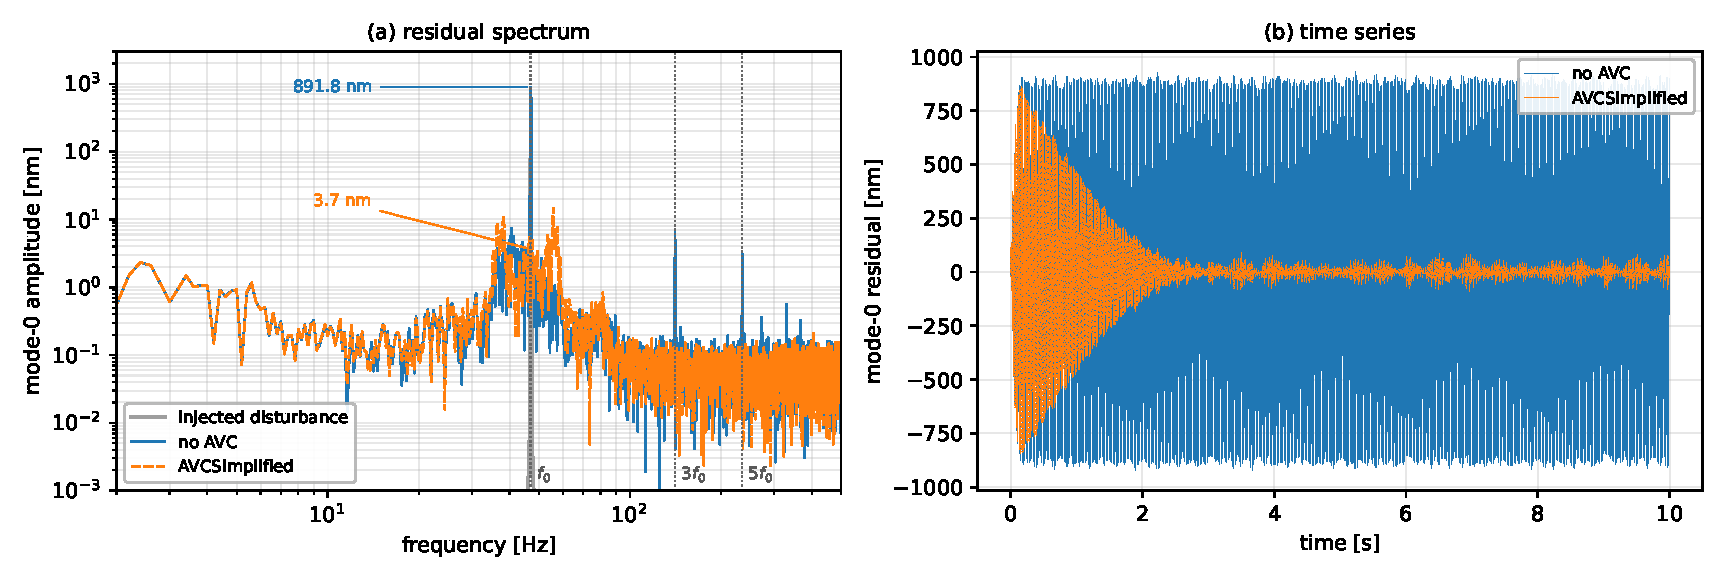
\includegraphics[width=\textwidth]{avc_simplified_psd.pdf}
\caption{Simplified AVC in closed loop. (a) Steady-state mode-0 spectrum with
the module off and on, against the injected disturbance (grey). (b) The same
run in the time domain; convergence takes about \SI{2}{s}, set by
$\tfrac12 g_x\,\mathrm{Re}\,\kappa$.}
\label{fig:simplpsd}
\end{figure}

\paragraph{Harmonics rejection.}
Figure~\ref{fig:simplpsd}(a) also shows how the AVC removes the odd harmonics of the vibration, for which there is no explicit rejection loop. Some results are collected in Table~\ref{tab:simplharmonics}. 
\begin{table}\small
\centering
\begin{tabular}{rrrrr}
\toprule
harmonic & $f$ [Hz] & injected & no AVC & with AVC\\
\midrule
1 & 47  & \SI{120}{nm} & \SI{891.8}{nm} & \SI{3.69}{nm}\\
3 & 141 & ---          & \SI{6.36}{nm}  & \SI{0.11}{nm}\\
5 & 235 & ---          & \SI{3.33}{nm}  & \SI{0.09}{nm}\\
7 & 329 & ---          & \SI{0.56}{nm}  & \SI{0.10}{nm}\\
\bottomrule
\end{tabular}
\caption{Rejection of Odd Harmonics with AVC on the fundamental}
\label{tab:simplharmonics}
\end{table}
\noindent
The odd harmonics have to be generated by an odd-symmetric nonlinearity in the loop. A reasonable guess for the generation of the odd harmonics is the WFS. 
%
Since the harmonics are generated by the nonlinearity in the sensor, the AVC does not need to be tuned to reject them: the rejection of the fundamental is enough to remove the harmonics as well.
%
\paragraph{Sweeping the calibration phase.}
The algorithm initialization must only satisfy the margin condition \eqref{eq:margin}: for testing, the calibration phase was offset by a controlled $\Delta\varphi$, everything else left unchanged, and the frequency held fixed at \SI{47}{Hz} so that the phase effect is not confounded with the PLL losing lock once the tone stops being cancelled. Figure~\ref{fig:simplmargin} and Table~\ref{tab:simplsweep} collect the result.
%
\begin{table}
\centering\small
\begin{tabular}{rrrl}
\toprule
$\Delta\varphi$ & mode-0 RMS & \SI{47}{Hz} amp. & behavior\\
\midrule
$-80^\circ$  & \SI{308}{nm}  & \SI{431}{nm}  & converges, slowly\\
$-68^\circ$  & \SI{131}{nm}  & \SI{174}{nm}  & converges\\
$-43^\circ$  & \SI{17.5}{nm} & \SI{9.2}{nm}  & converges\\
$0^\circ$    & \SI{14.8}{nm} & \SI{2.8}{nm}  & converges\\
$+47^\circ$  & \SI{15.0}{nm} & \SI{4.8}{nm}  & converges\\
$+77^\circ$  & \SI{240}{nm}  & \SI{320}{nm}  & converges, slowly\\
$+87^\circ$  & \SI{951}{nm}  & \SI{1284}{nm} & marginal\\
$+97^\circ$  & \SI{1380}{nm} & \SI{1882}{nm} & diverges\\
$+137^\circ$ & \SI{1269}{nm} & \SI{1662}{nm} & diverges\\
\bottomrule
\end{tabular}
\caption{Sweeping the calibration phase}
\label{tab:simplsweep}
\end{table}
%
\begin{figure}[t!]
\centering
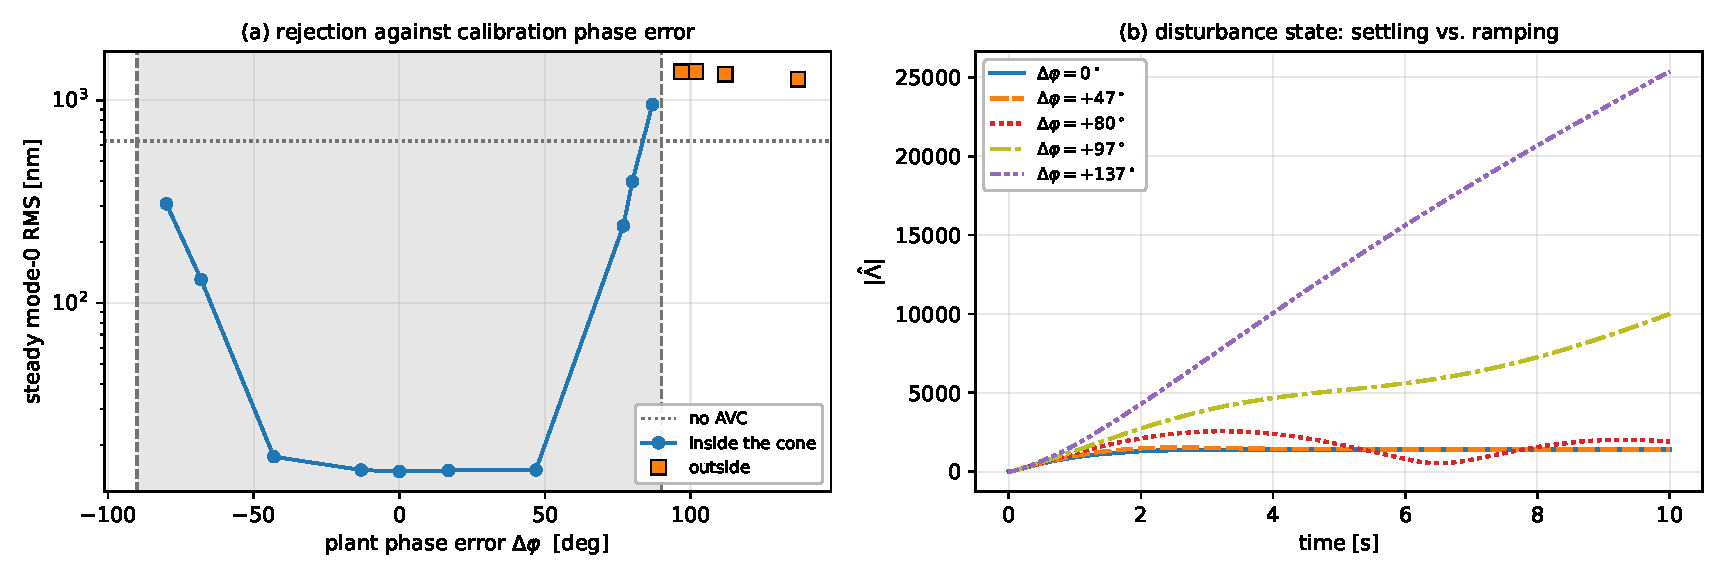
\includegraphics[width=\textwidth]{avc_simplified_margin.pdf}
\caption{The margin condition in the full simulation. (a) Steady mode-0 RMS against calibration phase error; the shaded band is the predicted cone \eqref{eq:margin} and the dotted line the residual without AVC. (b)
Trajectories of $|\hat\Lambda|$: settling inside the cone, and the unbounded ramp of the integrator outside it.}
\label{fig:simplmargin}
\end{figure}
%
As predicted from the theoretical analysis, the transition seems to happen at $\pm90^\circ$; the divergence rate is also influenced by the phase mismatch, with the integrator ramping faster the further outside the cone it is.
%
It should be noted that for a plant phase error close to $90^\circ$ the convergence is slow, and the residual is worse than the baseline. This may be a hint to some mismatch due to the calibration procedure, yet to be investigated.
% \newpage
\bibliographystyle{ieeetr}
\bibliography{avc_report}

\end{document}
